\begin{equation}
\langle \widetilde{\delta} ({\bf k}) \widetilde{\delta} ({\bf k'}) \rangle = (2 \pi) ^3 \delta_D \left( {\bf k} - {\bf k'} \right) P \left({\bf k} \right)
\end{equation}

We can estimate the power spectrum with the relational

\begin{equation}
P\left( k\right) \approx \frac{\sum_{\textbf{k} \in k}\langle | \widetilde{\delta} \left( \textbf{k}\right) |^2 \rangle}{N_k V}
\end{equation}

\begin{equation}
    \widetilde{\Delta}^2 \left( k \right) =  \left( k \right) \frac{k^3}{2 \pi ^2} P \left( k \right)
\end{equation}

\begin{equation}
    \Delta^2 \left( k \right) = \left( \nu \bar{I}_{\nu} \right)^2 \widetilde{\Delta}^2 \left( k \right)
\end{equation}s

\begin{figure}[ht]
	\centering
	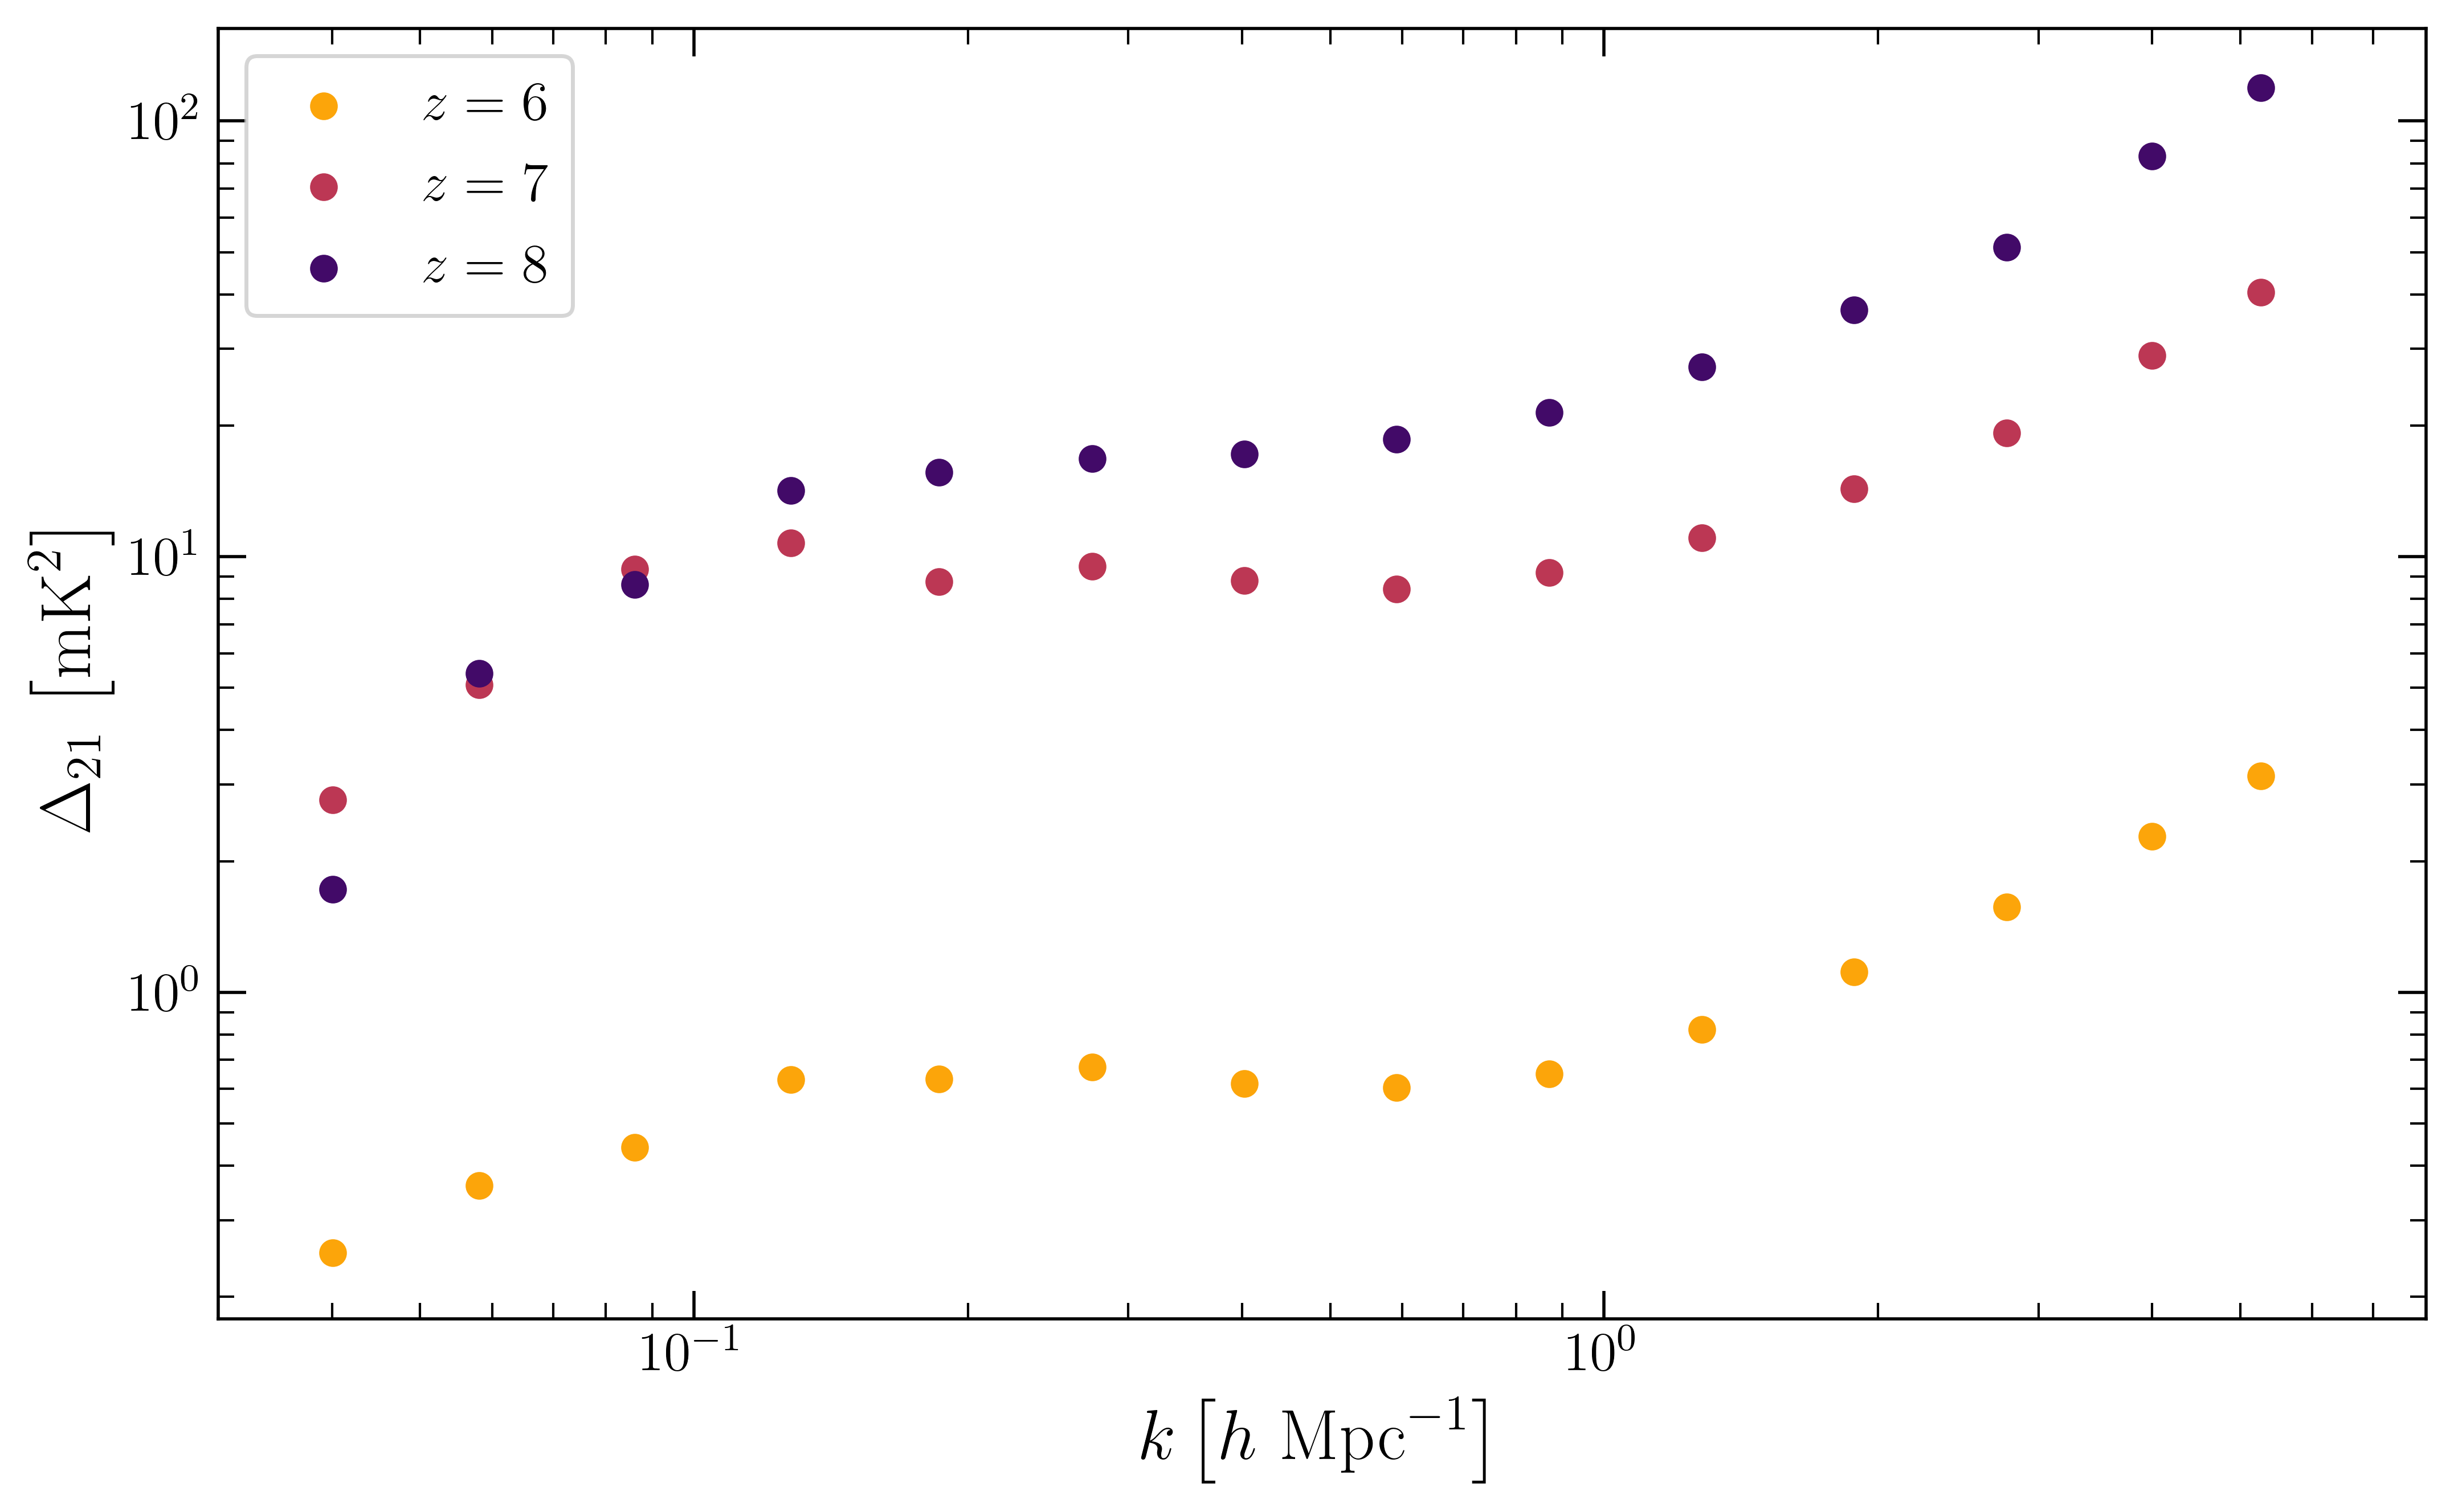
\includegraphics[width=1.\textwidth]{21cm_power_spectrum.png}
	\caption[21cm Power Spectrum]{Cross-correlation coefficient}
	\label{fig:21cm_ps}
\end{figure}

\begin{figure}[ht]
	\centering
	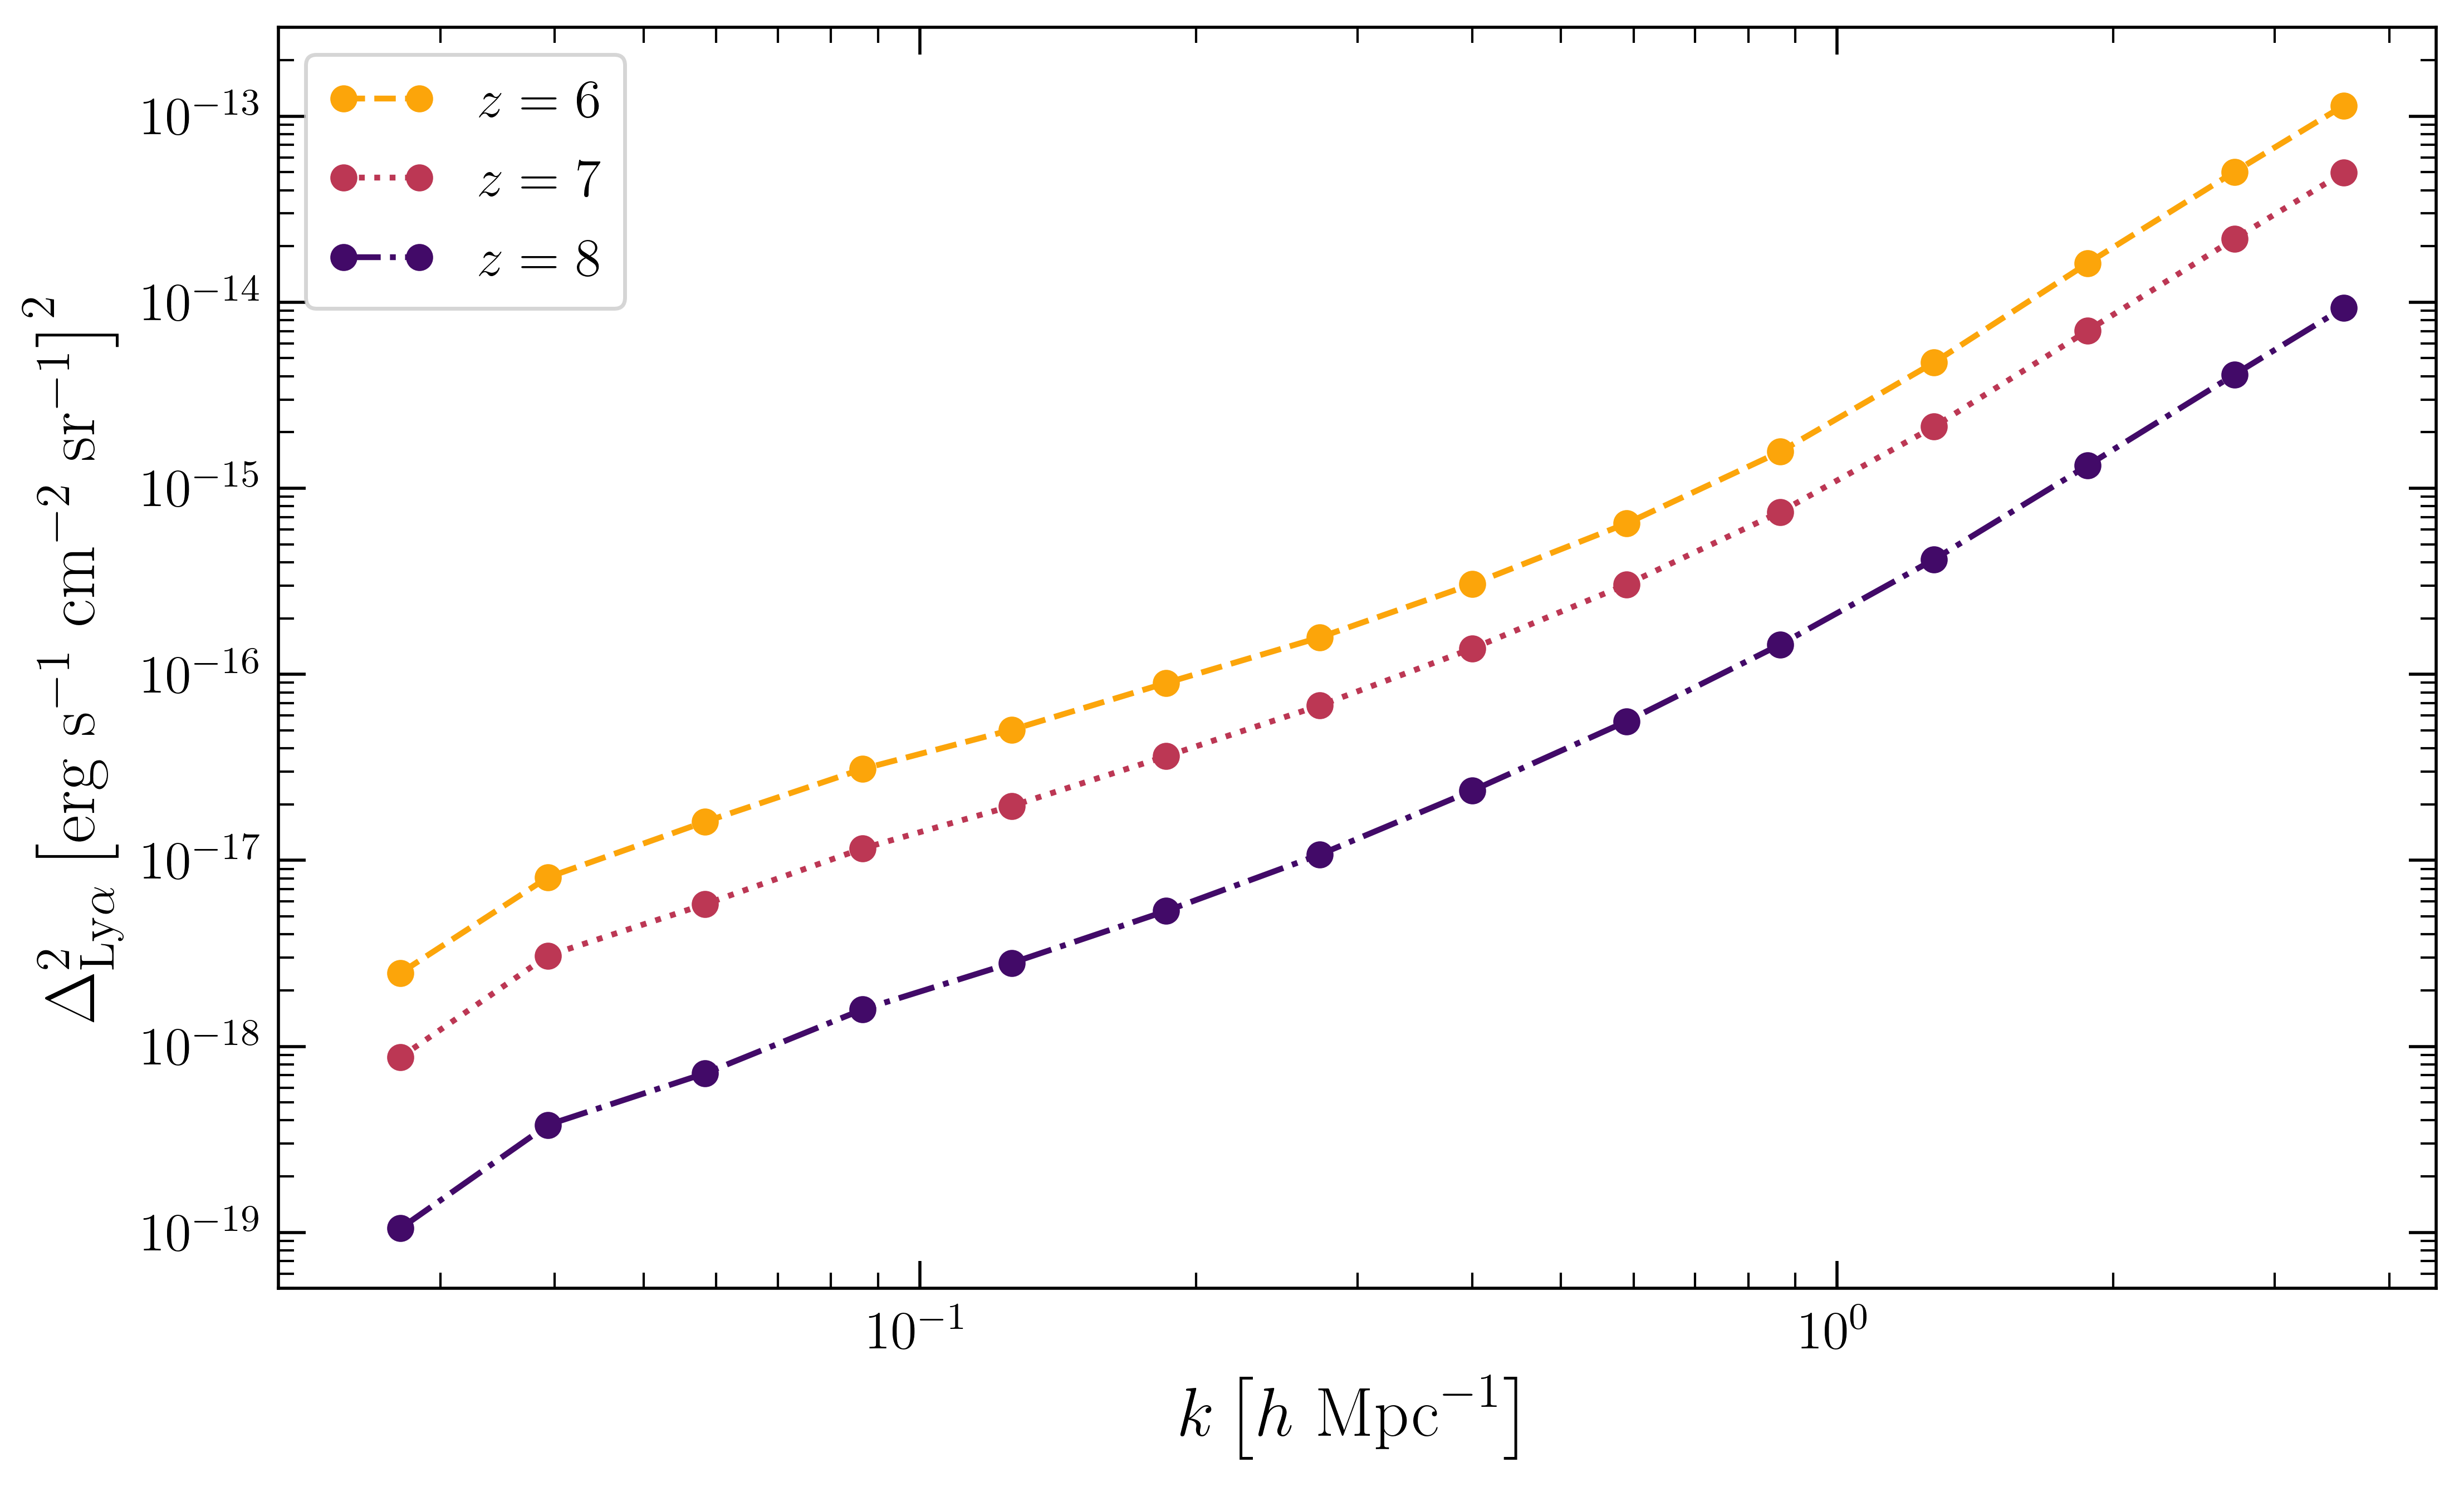
\includegraphics[width=1.\textwidth]{lyman_alpha_pspec.png}
	\caption[Ly$\alpha$ Power Spectrum]{Cross-correlation coefficient}
	\label{fig:lya_ps}
\end{figure}

\begin{figure}[ht]
	\centering
	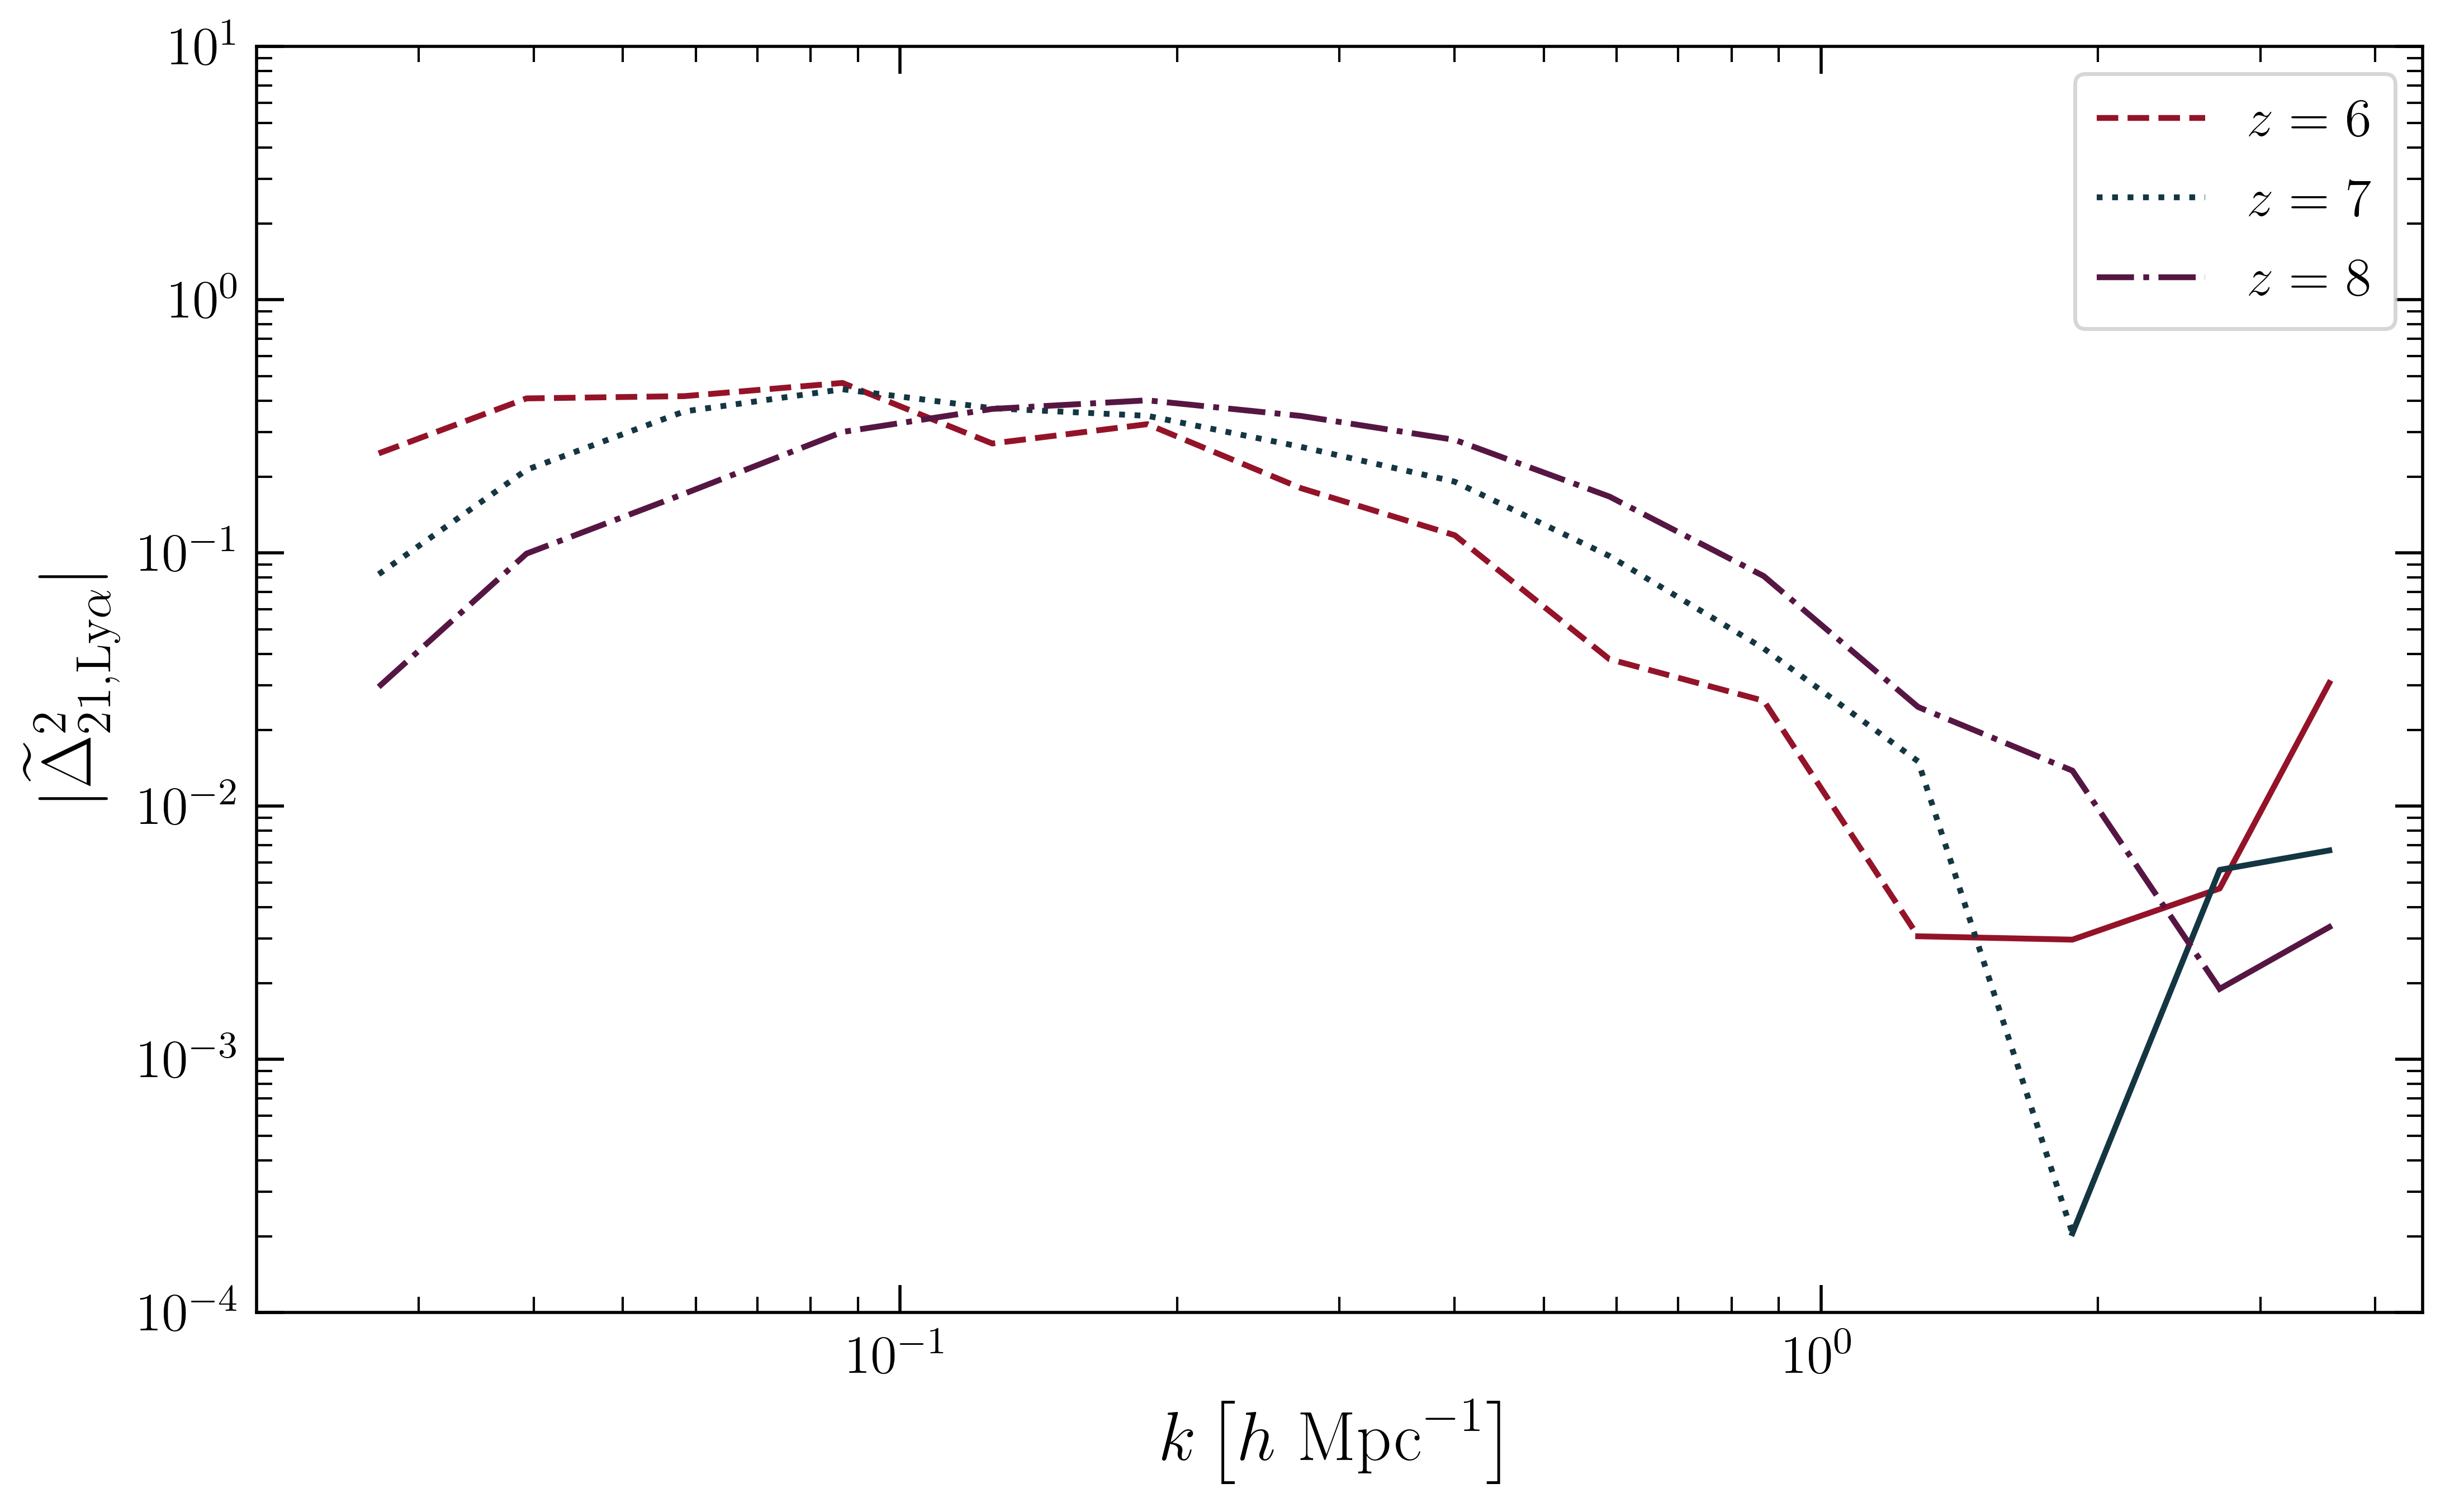
\includegraphics[width=1.\textwidth]{cross_power_spec.png}
	\caption[Cross-Power Spectrum]{Cross-correlation coefficient}
	\label{fig:x_ps}
\end{figure}

\begin{figure}[ht]
	\centering
	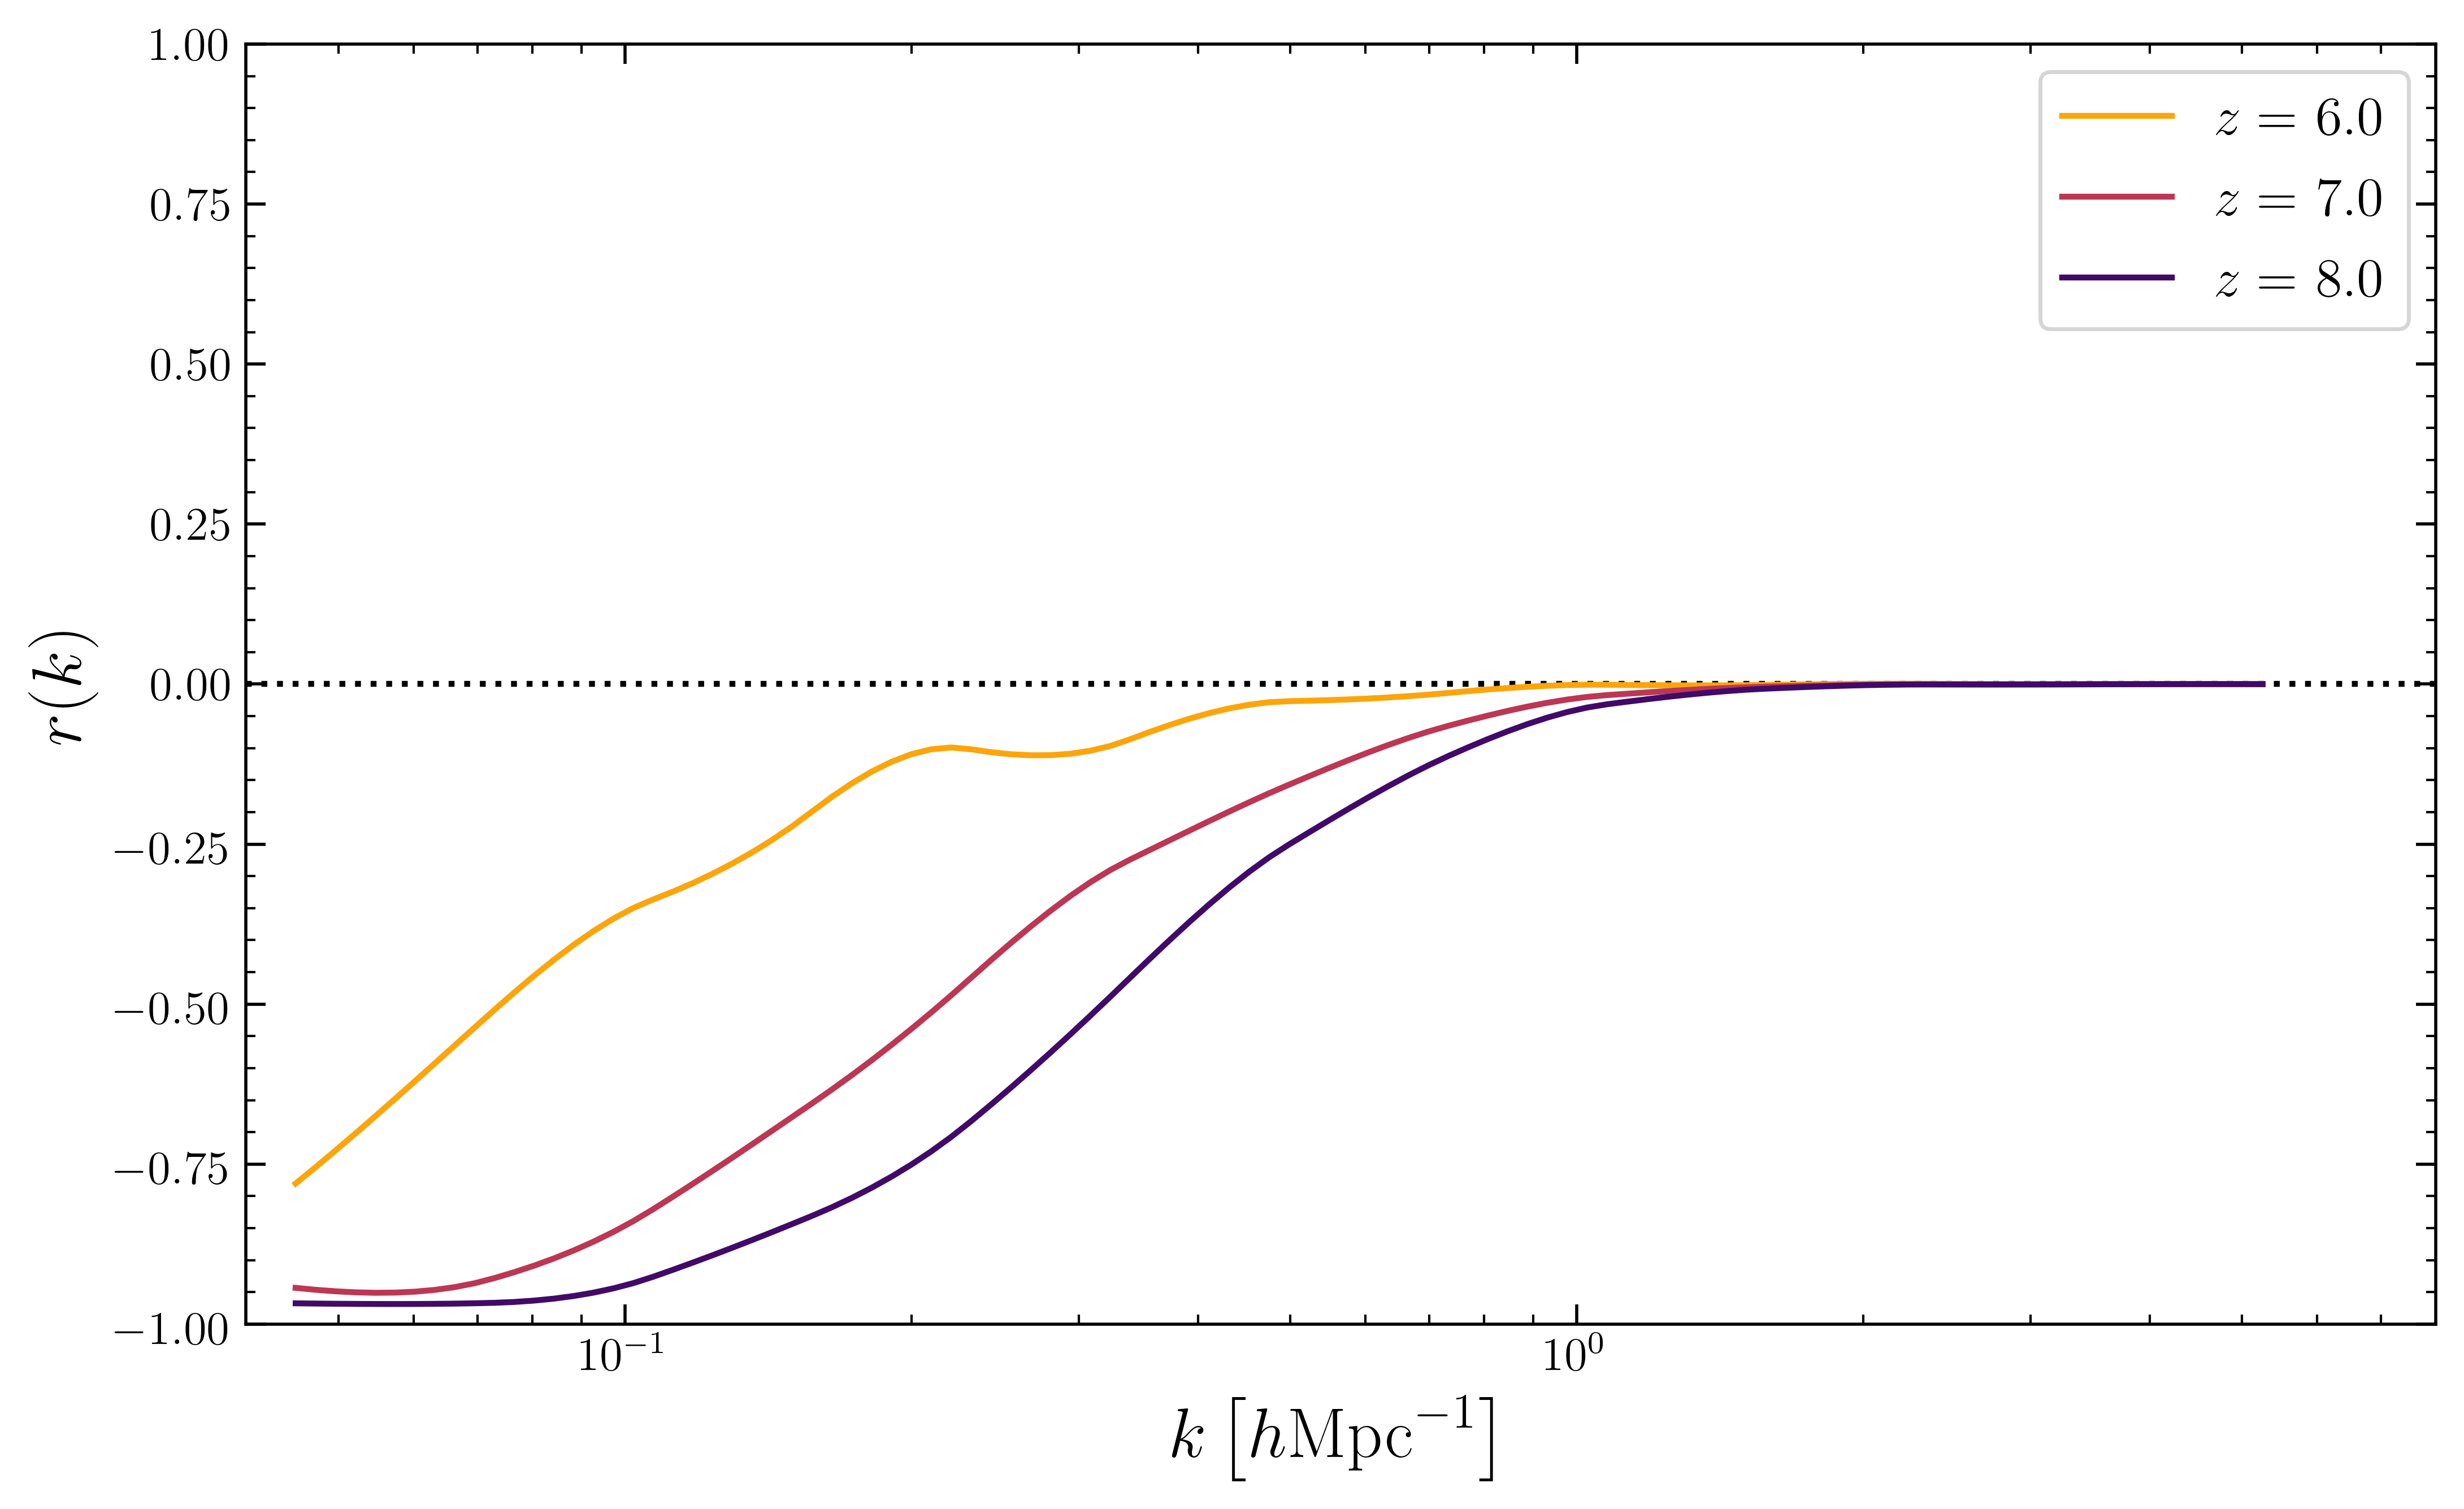
\includegraphics[width=1.\textwidth]{ccc_plot.png}
	\caption[Cross-Correlation Coefficient]{Cross-correlation coefficient}
	\label{fig:ccc}
\end{figure}
